% =====================================================
% TIÊU ĐỀ ĐỒ ÁN
% =====================================================

{\Large \bfseries Tiêu đề đồ án: Phát hiện bất thường trên endpoint device log dựa trên OCR-APT (Subgraph Anomaly Detection với One-Class RGCN)}

\vspace{1cm}

% =====================================================
% ABSTRACT
% =====================================================

\begin{abstract}
Đồ án nhắm tới một bài toán thực tế: phát hiện \emph{trực tiếp}, từ log nhân của một máy Windows, một cuộc tấn công phổ biến: kẻ tấn công khai thác lỗ hổng (CVE) của một dịch vụ web trong lab, thực thi mã từ xa (RCE), rồi chạy tiếp các kỹ thuật MITRE ATT\&CK (khám phá hệ thống, duy trì truy cập, đánh cắp thông tin xác thực, kênh điều khiển C2, rút dữ liệu). Log nhân ghi lại mọi tiến trình, tệp và kết nối mạng nên chứa dấu vết của chuỗi này, nhưng khối lượng rất lớn và không có nhãn tấn công để huấn luyện. Các hệ thống phát hiện bất thường hiện nay thường cảnh báo ở mức quá thô (cả đồ thị, cả cửa sổ thời gian) hoặc quá vụn (từng nút riêng lẻ), đồng thời phụ thuộc vào thuộc tính dễ giả mạo như đường dẫn tệp hay địa chỉ IP.

Đồ án lấy \emph{phương pháp} từ OCR-APT \cite{aly2025ocrapt}, một hệ thống vốn được thiết kế cho tấn công APT. OCR-APT biểu diễn log thành đồ thị nguồn gốc (provenance graph), trích đặc trưng hành vi cho từng nút, huấn luyện cho mỗi loại nút một mô hình one-class RGCN (OCRGCN) chỉ trên dữ liệu lành tính, gom các nút bất thường thành đồ thị con có điểm bất thường (Thuật toán 1), rồi dùng mô hình ngôn ngữ lớn (LLM) để dựng lại câu chuyện tấn công (Thuật toán 2). Vì mô hình chỉ học hành vi lành tính, nó gắn cờ mọi hành vi mà dữ liệu huấn luyện chưa từng có, nên không bị giới hạn ở APT.

Đồ án xây dựng lại phần lõi của OCR-APT dưới dạng một bản chứng minh khái niệm (proof of concept) chạy gần thời gian thực trên dữ liệu ETW do nhóm tự thu thập từ một máy Windows trong phòng lab: log được đẩy qua Grafana Alloy về Loki, chuyển sang lược đồ NODLINK Windows 10, cắt thành cửa sổ 5 phút, chấm điểm bằng OCRGCN tự hiện thực, lọc bằng điểm đồ thị con, và (tuỳ chọn) được LLM phân loại và viết báo cáo. Báo cáo trình bày lý thuyết cốt lõi của bài báo, các điểm nhóm làm khác bài báo cùng lý do và giới hạn kèm theo, và kết quả thực nghiệm. \todoval[Kết quả chính: số cửa sổ lành tính bị cảnh báo nhầm, cửa sổ tấn công có chuyển đỏ hay không, kết luận của LLM.]
\end{abstract}

\vspace{1cm}

% =====================================================
% MỤC TIÊU ĐỒ ÁN
% =====================================================

\section{Mục tiêu đồ án}

Mục tiêu của đồ án là:
\begin{itemize}
    \item Hiểu và trình bày được từng thành phần cốt lõi của OCR-APT: đồ thị nguồn gốc, đặc trưng hành vi, RGCN, học một lớp (one-class), mô hình theo loại nút, xây dựng đồ thị con bất thường và điều tra bằng LLM.
    \item Tự hiện thực lại phần lõi đó (khoảng 40\% hệ thống trong bài báo) thành một pipeline có thể kiểm tra từng bước: mỗi giai đoạn ghi ra CSV/JSON độc lập để phân tích (EDA).
    \item Trình diễn trực tiếp ý tưởng của bài báo: khi một cuộc tấn công thật (khai thác CVE trên dịch vụ lab $\rightarrow$ thực thi mã từ xa $\rightarrow$ các kỹ thuật MITRE ATT\&CK \cite{mitre_attack}) chạy trong buổi demo, cửa sổ chứa tấn công chuyển sang cảnh báo đỏ, còn các cửa sổ lành tính giữ màu xanh. Tấn công mục tiêu là một tấn công phổ biến, không phải APT: OCR-APT cung cấp phương pháp, không phải mô hình mối đe doạ.
    \item Ghi lại trung thực quan hệ với bài báo: phần nào tái hiện, phần nào điều chỉnh, phần nào bỏ qua, và những khẳng định nào vì thế không được phép đưa ra.
\end{itemize}

Đồ án \textbf{không} nhằm tái hiện các bảng số liệu của bài báo, không chạy lại các baseline (NODLINK, FLASH, \ldots) và không so sánh trực tiếp số liệu của nhóm với số liệu của bài báo, vì dữ liệu, nhãn và cách thiết lập khác nhau.

% =====================================================
% TỔNG QUAN NGHIÊN CỨU
% =====================================================

\section{Tổng quan nghiên cứu}
\label{sec:overview}

\paragraph{Bối cảnh và vấn đề.}
Một kịch bản xâm nhập máy trạm rất phổ biến là khai thác lỗ hổng của một dịch vụ hướng ra mạng (ATT\&CK T1190), lấy được quyền thực thi lệnh, rồi khám phá hệ thống, cài cơ chế duy trì, đánh cắp thông tin xác thực, mở kênh C2 và rút dữ liệu. Mỗi bước đều để lại dấu vết trong log của hệ điều hành: tiến trình nào sinh tiến trình nào, ghi tệp gì, kết nối tới đâu. Tấn công có chủ đích kéo dài (APT), động lực chính của bài báo OCR-APT, là trường hợp khó nhất của cùng bài toán này: nhiều giai đoạn, chậm và kín đáo. Đồ thị nguồn gốc (provenance graph) mô hình hoá các log này thành một đồ thị có hướng, không đồng nhất, trong đó nút là thực thể hệ thống và cạnh là hành động, cho phép lần theo quan hệ nhân quả mà log dạng tuyến tính làm mất \cite{zipperle2022survey}. Vấn đề là đồ thị này rất lớn (hàng triệu nút), còn phần liên quan tới tấn công chỉ chiếm dưới 0.01\% số nút trong các bộ dữ liệu chuẩn \tagpaper~\cite{aly2025ocrapt}.

\paragraph{Giới hạn của các hệ thống hiện có} \tagpaper~(§1--2 của bài báo).
\begin{itemize}
    \item \textbf{Dựa trên luật/chữ ký:} chỉ phát hiện được tấn công đã biết, không phát hiện được kỹ thuật mới.
    \item \textbf{Phát hiện bất thường ở mức quá thô hoặc quá vụn:} cảnh báo theo cả đồ thị hoặc cả cửa sổ thời gian thì khó điều tra (``mò kim đáy bể''); cảnh báo theo từng nút hoặc cạnh thì sinh nhiều cảnh báo rời rạc, thiếu ngữ cảnh, và tỉ lệ dương tính giả cao.
    \item \textbf{Phụ thuộc vào thuộc tính nút:} các hệ thống như NODLINK \cite{li2024nodlink}, FLASH \cite{rehman2024flash}, KAIROS \cite{cheng2024kairos} dùng tên tiến trình, dòng lệnh, đường dẫn tệp, địa chỉ IP để tạo embedding. Mô hình dễ học thuộc các chi tiết bề mặt này (spurious correlation \cite{arp2022dos}) và kẻ tấn công có thể đổi chúng mà không đổi hành vi.
    \item \textbf{Bỏ qua loại cạnh:} nhiều mô hình GNN trước đây (ví dụ dựa trên GraphSAGE như ThreaTrace \cite{wang2022threatrace}) được thiết kế cho đồ thị đồng nhất, không phân biệt ``đọc'' với ``ghi'' hay ``khởi chạy''.
    \item \textbf{Điều tra sau cảnh báo:} nhiều hệ thống cần điểm bắt đầu do người phân tích chỉ định (POI) và chỉ xuất ra đồ thị hoặc chuỗi sự kiện mức thấp, khó đọc.
\end{itemize}

\paragraph{Hướng tiếp cận của OCR-APT.}
OCR-APT giải quyết các điểm trên bằng: (i) đặc trưng hành vi và cấu trúc thay vì thuộc tính nút; (ii) RGCN để giữ loại cạnh khi tổng hợp thông tin láng giềng; (iii) học một lớp chỉ trên dữ liệu lành tính, không cần nhãn tấn công; (iv) một mô hình cho mỗi loại nút; (v) gom nút bất thường thành đồ thị con và lọc theo điểm bất thường của đồ thị con; (vi) một pipeline LLM nhiều bước có kiểm tra ảo giác để viết báo cáo tấn công. Trên DARPA TC3 \cite{darpa_tc3}, DARPA OpTC \cite{darpa_optc} và tập NODLINK mô phỏng \cite{nodlink_data}, bài báo báo cáo độ chính xác ngang hoặc cao hơn các hệ thống hiện có \tagpaper.

\paragraph{Từ APT sang tấn công phổ biến.}
Đồ án dùng phương pháp của OCR-APT cho một tấn công phổ biến chứ không cho APT. Lý do phương pháp vẫn áp dụng được:
\begin{itemize}
    \item Mô hình một lớp chỉ học hành vi lành tính, không học dấu hiệu của một loại tấn công cụ thể. Bất kỳ hành vi nào dữ liệu huấn luyện chưa từng có đều có thể gây cảnh báo, dù là APT hay không.
    \item Một chuỗi sau RCE (dịch vụ web sinh ra shell, thả tệp, kết nối ra ngoài) diễn ra nhanh và để lại nhiều cạnh bất thường gần nhau trong đồ thị. \taginf{} Với bộ phát hiện này, nó dễ hơn một APT ``low and slow''.
    \item Một số phần của bài báo gắn chặt với APT trở nên ít trung tâm hơn: lập luận ``nút APT nghỉ lâu hơn'' cho đặc trưng thời gian nghỉ (Mục~\ref{sec:theory-features}), và báo cáo theo giai đoạn kill chain của APT, mà đồ án ánh xạ sang tactic ATT\&CK (Mục~\ref{sec:dev-llm}).
\end{itemize}

\paragraph{Khoảng trống và câu hỏi của đồ án.}
Bài báo đánh giá OCR-APT ngoại tuyến (offline) trên toàn bộ log của các bộ dữ liệu công bố sẵn. Đồ án đặt câu hỏi: \emph{ý tưởng cốt lõi đó có hoạt động được khi chạy gần thời gian thực, theo từng cửa sổ 5 phút, trên dữ liệu Windows do chính nhóm thu thập hay không?} Cụ thể:
\begin{itemize}
    \item \textbf{RQ1:} Với hoạt động lành tính, các cửa sổ có giữ được trạng thái xanh (không có đồ thị con nào đạt mức cảnh báo) không?
    \item \textbf{RQ2:} Khi một cuộc tấn công thật (khai thác CVE $\rightarrow$ RCE $\rightarrow$ các kỹ thuật ATT\&CK) chạy trong lúc demo, cửa sổ chứa tấn công có chuyển đỏ, và đồ thị con cảnh báo có chứa các thực thể của tấn công không?
    \item \textbf{RQ3:} LLM có phân biệt được cảnh báo thật với cảnh báo nhầm và viết lại được diễn biến tấn công từ đồ thị con không?
\end{itemize}

% =====================================================
% CƠ SỞ LÝ THUYẾT
% =====================================================

\section{Cơ sở lý thuyết}
\label{sec:theory}

Phần này trình bày các thành phần cốt lõi của OCR-APT theo thứ tự dữ liệu đi qua hệ thống (Hình~\ref{fig:ocrapt-arch}). Mỗi công thức đi kèm kích thước tensor và ví dụ số cụ thể. Các nhãn \tagpaper, \tagrepo, \tagours, \taginf{} cho biết phát biểu đến từ bài báo, từ mã nguồn gốc \cite{ocrapt_repo}, từ nhóm, hay là suy luận chưa kiểm chứng.

\begin{figure}[H]
\centering
\begin{tikzpicture}
  \node[anchor=south west, inner sep=0] (img) at (0,0) {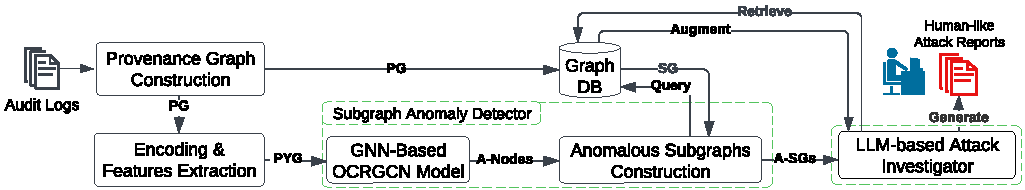
\includegraphics[width=\textwidth]{images/paper-fig1-architecture.pdf}};
  \begin{scope}[x={(img.south east)}, y={(img.north west)}]  % (0,0) = góc dưới trái, (1,1) = góc trên phải của ảnh
    \node[num] at (0.085, 0.84) {1};
    \node[num] at (0.103, 0.37) {2};
    \node[num] at (0.312, 0.33) {3};
    \node[num] at (0.540, 0.33) {4};
    \node[num] at (0.812, 0.33) {5};
  \end{scope}
\end{tikzpicture}
\caption{\textbf{Log thô đi vào, báo cáo tấn công đi ra, qua 5 bước.} Đọc theo số: \stepnum{1} dựng đồ thị nguồn gốc từ audit log; \stepnum{2} mã hoá đồ thị và trích đặc trưng hành vi; \stepnum{3} mô hình OCRGCN chấm điểm từng nút; \stepnum{4} gom các nút bất thường thành đồ thị con và lọc theo điểm; \stepnum{5} LLM viết báo cáo tấn công. Mỗi số tương ứng với một mục của phần này (\stepnum{1}~Mục~\ref{sec:theory-pg}, \stepnum{2}~Mục~\ref{sec:theory-features}, \stepnum{3}~Mục~\ref{sec:theory-rgcn}--\ref{sec:theory-tsmod}, \stepnum{4}~Mục~\ref{sec:theory-alg1}, \stepnum{5}~Mục~\ref{sec:theory-llm}). Nguồn: Hình~1 của \cite{aly2025ocrapt}, số thứ tự do nhóm thêm vào.}
\figlegend{\textbf{Chú giải:} khung xanh lá nét đứt lớn = bộ phát hiện đồ thị con bất thường (bước \stepnum{3}+\stepnum{4}); \emph{PG} = đồ thị nguồn gốc; \emph{PYG} = đồ thị đã mã hoá cho PyTorch Geometric; \emph{A-Nodes} = các nút bất thường; \emph{A-SGs} = các đồ thị con bất thường; \emph{SG}/\emph{Query} = truy vấn đồ thị con từ Graph DB; \emph{Retrieve}/\emph{Augment} = LLM lấy thêm ngữ cảnh từ Graph DB để bổ sung báo cáo.}
\label{fig:ocrapt-arch}
\end{figure}

% -----------------------------------------------------
\subsection{Đồ thị nguồn gốc và mô hình mối đe doạ}
\label{sec:theory-pg}

\paragraph{Định nghĩa.}
Đồ thị nguồn gốc $G = (V, E)$ là đồ thị có hướng, không đồng nhất \tagpaper~(§2):
\begin{itemize}
    \item Mỗi nút $v \in V$ là một thực thể hệ thống và có đúng một \textbf{loại nút} $\tau(v)$. Với dữ liệu Windows 10 mô phỏng của NODLINK, có ba loại: \texttt{PROCESS}, \texttt{FILE}, \texttt{NET} (luồng mạng) \tagrepo.
    \item Mỗi cạnh $(u, r, v) \in E$ là một hành động có \textbf{loại cạnh} (quan hệ) $r$ và dấu thời gian. Windows 10 của NODLINK có 6 loại: \texttt{Start}, \texttt{Load}, \texttt{Read}, \texttt{Write}, \texttt{Send}, \texttt{Recv}. Chủ thể $u$ luôn là một tiến trình.
    \item Nút còn có thuộc tính (tên tiến trình, đường dẫn, IP:cổng). OCR-APT \emph{không} đưa thuộc tính vào mô hình mà chỉ giữ lại cho bước điều tra \tagpaper~(§5.1.1).
\end{itemize}
OCR-APT lưu đồ thị dưới dạng RDF, tức tập bộ ba $\langle$subject, predicate, object$\rangle$, ví dụ $\langle$\texttt{proc:4012}, \texttt{Write}, \texttt{file:payload.exe}$\rangle$, trong một cơ sở dữ liệu đồ thị (GraphDB \cite{graphdb}), để truy vấn đồ thị con mà không phải nạp cả đồ thị vào bộ nhớ.

\begin{figure}[H]
\centering
\begin{tikzpicture}[
  proc/.style={draw, rectangle, rounded corners, fill=white, font=\small\ttfamily, minimum height=0.7cm},
  file/.style={draw, ellipse, fill=white, font=\small\ttfamily},
  net/.style={draw, diamond, aspect=2.2, fill=white, font=\small\ttfamily, inner sep=1pt},
  atk/.style={-{Stealth[length=2.2mm]}, very thick, catk},
  ben/.style={-{Stealth[length=2mm]}, gray},
  lab/.style={font=\scriptsize, midway, fill=white, inner sep=1pt},
  t/.style={circle, fill=catk, text=white, font=\tiny\bfseries, inner sep=1pt}]
  \node[proc] (svc) at (0,0) {node.exe};
  \node[proc] (cmd) at (3.6,0) {cmd.exe};
  \node[proc] (ps)  at (7.2,0) {powershell.exe};
  \node[net]  (c2)  at (11,0.9) {10.0.0.5:443};
  \node[file] (pay) at (11,-0.9) {payload.exe};
  \node[file] (dll) at (3.6,-1.7) {ntdll.dll};
  \draw[atk] (svc) -- node[lab]{Start} node[t, above=3pt]{1} (cmd);
  \draw[atk] (cmd) -- node[lab]{Start} node[t, above=3pt]{2} (ps);
  \draw[atk] (ps) -- node[lab, sloped]{Send} node[t, above=4pt]{3} (c2);
  \draw[atk] (c2) to[bend left=20] node[lab]{Recv} (ps);
  \draw[atk] (ps) -- node[lab, sloped]{Write} node[t, below=4pt]{4} (pay);
  \draw[ben] (cmd) -- node[lab]{Load} (dll);
\end{tikzpicture}
\caption{\textbf{Một cuộc tấn công nhìn dưới dạng đồ thị.} Đọc theo số đỏ: \textcolor{catk}{1} dịch vụ web \texttt{node.exe} bị khai thác RCE và sinh ra \texttt{cmd.exe} (một ``cha bất thường''); \textcolor{catk}{2} \texttt{cmd.exe} mở \texttt{powershell.exe}; \textcolor{catk}{3} PowerShell kết nối tới máy chủ C2; \textcolor{catk}{4} PowerShell thả tệp \texttt{payload.exe}. Cạnh xám là hoạt động bình thường mà tiến trình nào cũng có. Đồ thị minh hoạ của nhóm theo lược đồ Windows 10 của NODLINK.}
\figlegend{\textbf{Chú giải:}
  \tikz[baseline=-0.6ex]\node[draw, rounded corners, minimum width=0.6cm, minimum height=0.3cm]{};~tiến trình (\texttt{PROCESS})\quad
  \tikz[baseline=-0.6ex]\node[draw, ellipse, minimum width=0.6cm, minimum height=0.3cm]{};~tệp (\texttt{FILE})\quad
  \tikz[baseline=-0.6ex]\node[draw, diamond, aspect=2, minimum width=0.6cm, minimum height=0.3cm, inner sep=0]{};~luồng mạng (\texttt{NET})\quad
  \arrowkey{-{Stealth[length=2mm]}, very thick, catk}{bước tấn công (số = thứ tự thời gian)}\quad
  \arrowkey{-{Stealth[length=2mm]}, gray}{hoạt động bình thường}. Nhãn trên cạnh là loại hành động; chủ thể của mọi cạnh là tiến trình (cạnh \texttt{Recv} vẽ ngược chiều để thể hiện luồng dữ liệu).}
\label{fig:pg-example}
\end{figure}

\paragraph{Mô hình mối đe doạ} \tagpaper~(§3).
Kẻ tấn công có thể dùng khai thác zero-day, nhưng phải để lại dấu vết trong log hệ thống. Log dùng để huấn luyện được giả định \textbf{không chứa dấu vết tấn công}. Hệ thống ghi log ở mức nhân được coi là đáng tin (thuộc trusted computing base). Đầu độc dữ liệu, tấn công phần cứng và kênh kề nằm ngoài phạm vi. Giả định ``log huấn luyện sạch'' là lý do đồ án không bao giờ đưa kết quả của LLM ngược lại làm dữ liệu huấn luyện (Mục~\ref{sec:dev-llm}).

% -----------------------------------------------------
\subsection{Đặc trưng hành vi của nút}
\label{sec:theory-features}

Thay vì thuộc tính, mỗi nút được mô tả bằng \emph{nó làm gì} và \emph{nó nghỉ bao lâu giữa các hành động} \tagpaper~(§5.1.2).

\paragraph{Tần suất hành động, chuẩn hoá L2.}
Với 6 loại cạnh và 2 chiều (nút là nguồn: \texttt{out}, nút là đích: \texttt{in}), mỗi nút có vectơ đếm $\mathbf{a} \in \mathbb{R}^{12}$, ví dụ $a_{\text{out\_send}}$ là số lần nút gửi dữ liệu. Vectơ này được chuẩn hoá L2 (chia cho độ dài Euclid):
\[
\hat{\mathbf{a}} = \frac{\mathbf{a}}{\|\mathbf{a}\|_2}, \qquad \|\mathbf{a}\|_2 = \sqrt{a_1^2 + a_2^2 + \dots + a_{12}^2}.
\]
Sau chuẩn hoá, tổng bình phương các thành phần bằng 1, nên vectơ chỉ còn mang \emph{tỉ lệ} giữa các hành động, không còn mang khối lượng hoạt động.
\begin{itemize}
    \item \emph{Ví dụ 1 (trình duyệt bận):} \texttt{out\_send} $= 300$, \texttt{out\_recv} $= 400$, còn lại bằng 0. $\|\mathbf{a}\|_2 = \sqrt{300^2 + 400^2} = 500$, nên $\hat{\mathbf{a}}$ có \texttt{out\_send} $= 0.6$, \texttt{out\_recv} $= 0.8$.
    \item \emph{Ví dụ 2 (cùng trình duyệt, lúc rảnh):} \texttt{out\_send} $= 3$, \texttt{out\_recv} $= 4$. $\|\mathbf{a}\|_2 = 5$, vẫn ra $(0.6, 0.8)$. Hai trạng thái có cùng hành vi nên có cùng đặc trưng, đúng như bài báo mong muốn (một trình duyệt mở nhiều kết nối vẫn là bình thường nếu tỉ lệ gửi/nhận bình thường).
    \item \emph{Ví dụ 3 (tiến trình thả tệp):} \texttt{out\_write} $= 3$, \texttt{out\_start} $= 4$. Cũng ra $0.6$ và $0.8$ nhưng ở \emph{hai cột khác}, nên là một điểm khác hẳn trong không gian đặc trưng.
\end{itemize}

\paragraph{Thống kê thời gian nghỉ, chuẩn hoá min-max.}
Sắp các dấu thời gian của mọi cạnh chạm tới nút theo thứ tự, lấy khoảng cách giữa hai sự kiện liên tiếp (giây); nút có 3 đặc trưng: nhỏ nhất, lớn nhất, trung bình của các khoảng nghỉ. Mỗi đặc trưng được đưa về khoảng $[0, 1]$ bằng
\[
x' = \frac{x - x_{\min}}{x_{\max} - x_{\min}},
\]
trong đó $x_{\min}, x_{\max}$ lấy trên tập dữ liệu. Bài báo lập luận rằng nút liên quan tới APT thường nghỉ lâu hơn nút lành tính (``low and slow''), nên các thống kê này là tín hiệu quan trọng \tagpaper. Với tấn công mục tiêu của đồ án thì khác: một chuỗi sau RCE chạy nhanh, nên có thể cho khoảng nghỉ \emph{ngắn} hoặc một tổ hợp hành động chưa từng thấy hơn là khoảng nghỉ dài; khi đó các tỉ lệ hành động được kỳ vọng mang phần lớn tín hiệu \taginf.
\begin{itemize}
    \item \emph{Ví dụ 1:} một tiến trình có sự kiện ở giây 0, 2, 3, 9. Khoảng nghỉ là 2, 1, 6, nên min $= 1$, max $= 6$, trung bình $= 3$. Nếu trên tập huấn luyện max-idle nằm trong $[0, 290]$ giây thì max-idle chuẩn hoá $= 6/290 \approx 0.021$.
    \item \emph{Ví dụ 2:} một tiến trình nằm im 145 giây giữa hai sự kiện có max-idle chuẩn hoá $= 145/290 = 0.5$. Nếu trong dữ liệu kiểm thử một nút nghỉ 300 giây thì giá trị là $300/290 \approx 1.034$, \emph{vượt khỏi} $[0, 1]$, vì thang đo cố định theo tập huấn luyện (Mục~\ref{sec:dev-features}).
\end{itemize}

Ghép lại, mỗi nút có vectơ đặc trưng $\mathbf{x}_i \in \mathbb{R}^{15}$ (12 tỉ lệ hành động + 3 thống kê nghỉ). Ma trận đặc trưng của cả đồ thị có kích thước $X \in \mathbb{R}^{[N, 15]}$ với $N$ là số nút. Bài báo cho thấy bỏ các đặc trưng này (biến thể \emph{Without B-Feat}, dùng đặc trưng kiểu ThreaTrace) làm mô hình không phát hiện được nút bất thường nào trên host WS12 \tagpaper~(Bảng~4).

% -----------------------------------------------------
\subsection{Mạng nơ-ron đồ thị và RGCN}
\label{sec:theory-rgcn}

\paragraph{Trực giác: truyền thông điệp.}
Đặc trưng riêng của một nút chưa đủ: một tệp \texttt{payload.exe} chỉ đáng ngờ khi biết \emph{ai} ghi nó và \emph{ai} chạy nó. Mạng nơ-ron đồ thị (GNN) giải quyết bằng truyền thông điệp: ở mỗi lớp, mỗi nút thu thập biểu diễn của láng giềng một bước, biến đổi chúng, cộng với biểu diễn của chính nó. Sau $L$ lớp, biểu diễn của nút mang thông tin từ vùng lân cận $L$ bước \cite{kipf2017gcn}. OCR-APT dùng $L = 3$ \tagpaper~(§7.2.1).

\paragraph{RGCN: một ma trận trọng số cho mỗi loại cạnh.}
GCN thông thường dùng chung một ma trận trọng số cho mọi láng giềng, nên ``ghi vào tệp'' và ``đọc tệp'' bị trộn như nhau. RGCN \cite{schlichtkrull2018rgcn} dùng riêng một ma trận $W_r$ cho mỗi quan hệ $r$:
\[
\mathbf{h}_i^{(l+1)} = \sigma\Big( W_0^{(l)} \mathbf{h}_i^{(l)} + \sum_{r \in \mathcal{R}} \sum_{j \in \mathcal{N}_i^r} \frac{1}{c_{i,r}} W_r^{(l)} \mathbf{h}_j^{(l)} \Big)
\]
Giải thích từng ký hiệu:
\begin{itemize}
    \item $\mathbf{h}_i^{(l)}$: biểu diễn của nút $i$ ở lớp $l$; $\mathbf{h}_i^{(0)} = \mathbf{x}_i$ (15 chiều).
    \item $\mathcal{R}$: tập quan hệ; $\mathcal{N}_i^r$: các láng giềng nối với $i$ qua quan hệ $r$.
    \item $c_{i,r} = |\mathcal{N}_i^r|$: hằng số chuẩn hoá, tức lấy \emph{trung bình} các láng giềng cùng quan hệ, để nút có nhiều láng giềng không lấn át.
    \item $W_0$: ma trận cho chính nút (self-loop); $W_r$: ma trận của quan hệ $r$; $\sigma$: hàm kích hoạt (ReLU, $\max(0, z)$).
\end{itemize}
Kích thước: lớp đầu $W_r \in \mathbb{R}^{[15, 32]}$, các lớp sau $\mathbb{R}^{[32, 32]}$, nên $H^{(0)} \in \mathbb{R}^{[N, 15]} \rightarrow H^{(1)} \in \mathbb{R}^{[N, 32]} \rightarrow H^{(2)} \rightarrow H^{(3)} = Z \in \mathbb{R}^{[N, 32]}$. Mã nguồn gốc thêm một quan hệ ngược \texttt{inv\_}$r$ cho mỗi quan hệ thuận để thông điệp đi được cả hai chiều \tagrepo, nên với 6 bộ ba (nguồn, cạnh, đích) xuất hiện trong dữ liệu ta có $|\mathcal{R}| = 12$.

\paragraph{Ví dụ số (đặc trưng 1 chiều cho dễ tính).}
Tiến trình $P$ có $h_P = 1$; ghi vào hai tệp có $h = 2$ và $h = 4$; gửi tới một nút mạng có $h = 10$. Giả sử $W_0 = 0.5$, $W_{\text{write}} = 0.1$, $W_{\text{send}} = 0.02$.
\begin{itemize}
    \item \emph{Ví dụ 1:} phần Write là trung bình $(2 + 4)/2 = 3$, nhân $0.1$ được $0.3$; phần Send là $10 \times 0.02 = 0.2$; phần bản thân là $1 \times 0.5 = 0.5$. Tổng $1.0$, qua ReLU vẫn là $h_P' = 1.0$.
    \item \emph{Ví dụ 2:} cùng các láng giềng đó nhưng hai tệp được \emph{nạp} (\texttt{Load}) thay vì ghi, với $W_{\text{load}} = -0.2$: phần Load là $3 \times (-0.2) = -0.6$, tổng $0.5 - 0.6 + 0.2 = 0.1$. Cùng láng giềng, cùng đặc trưng, nhưng loại cạnh khác cho biểu diễn khác. Đây là lý do bài báo chọn RGCN.
\end{itemize}

\paragraph{Phác thảo PyG.} Đoạn mã~\ref{lst:rgcn} là bộ mã hoá ba lớp, ghi kích thước tensor trong chú thích.

\begin{lstlisting}[language=Python, label={lst:rgcn}, caption={Bộ mã hoá RGCN 3 lớp với PyTorch Geometric \cite{fey2019pyg}.}]
from torch_geometric.nn import RGCNConv
convs = [RGCNConv(15, 32, num_relations=12),   # x [N,15] -> [N,32]
         RGCNConv(32, 32, num_relations=12),   # [N,32]  -> [N,32]
         RGCNConv(32, 32, num_relations=12)]   # [N,32]  -> z [N,32]
h = x
for k, conv in enumerate(convs):
    h = conv(h, edge_index, edge_type)         # edge_index [2,E], edge_type [E]
    if k < 2: h = h.relu()
\end{lstlisting}

% -----------------------------------------------------
\subsection{Học một lớp: siêu cầu bao dữ liệu lành tính}
\label{sec:theory-oneclass}

\paragraph{Trực giác.}
Không có nhãn tấn công nên không thể huấn luyện bộ phân loại hai lớp. Học một lớp (one-class) chỉ học ``bình thường trông như thế nào'': tìm một siêu cầu (hình cầu trong không gian 32 chiều) có tâm $\mathbf{c}$ và bán kính $R$ bao phần lớn embedding lành tính. Nút nằm xa tâm hơn bán kính là bất thường. Ý tưởng này xuất phát từ One-Class SVM \cite{schoelkopf2001ocsvm} và Deep SVDD \cite{ruff2018deepsvdd}; OCGNN \cite{wang2021ocgnn} áp dụng nó cho GNN trên đồ thị đồng nhất. OCRGCN của OCR-APT là phiên bản với bộ mã hoá RGCN, xây trên thư viện PyGOD \cite{liu2024pygod} \tagpaper.

\paragraph{Điểm bất thường.}
Với embedding $\mathbf{z}_i \in \mathbb{R}^{32}$ (một hàng của $Z$):
\[
s_i = \|\mathbf{z}_i - \mathbf{c}\|_2^2 - R^2 .
\]
$s_i > 0$ nghĩa là nút nằm ngoài siêu cầu.
\begin{itemize}
    \item \emph{Ví dụ 1:} trong 2 chiều cho dễ hình dung, $\mathbf{c} = (0, 0)$, $R = 1$, $\mathbf{z} = (0.6, 0.8)$: $\|\mathbf{z} - \mathbf{c}\|^2 = 0.36 + 0.64 = 1$, nên $s = 1 - 1 = 0$, nằm đúng trên mặt cầu.
    \item \emph{Ví dụ 2:} $\mathbf{z} = (3, 4)$: $\|\mathbf{z} - \mathbf{c}\|^2 = 9 + 16 = 25$, nên $s = 24 > 0$, bất thường.
\end{itemize}

\begin{figure}[H]
\centering
\begin{tikzpicture}[scale=0.95,
  ben/.style={circle, fill=gray!70, inner sep=1.3pt},
  lbl/.style={font=\scriptsize, align=left}]
  % mặt cầu học được (R = 1) và ngưỡng theta (lớn hơn một chút)
  \fill[cdet] (0,0) circle (1);
  \draw[thick, blue!60!black] (0,0) circle (1);
  \draw[densely dotted, thick] (0,0) circle (1.3);
  % nút lành tính: phần lớn nằm trong, vài nút nằm ngoài nhưng dưới ngưỡng
  \foreach \p in {(0.2,0.3),(-0.4,0.1),(0.1,-0.5),(-0.2,-0.3),(0.5,-0.1),(-0.6,0.5),(0.3,0.6),(-0.1,0.7),(-0.7,-0.4),(0.6,-0.6)}
    \node[ben] at \p {};
  \node[ben] at (1.05,0.3) {}; \node[ben] at (-0.95,-0.55) {};
  % tâm và bán kính
  \node[circle, fill=black, inner sep=1.2pt, label={[font=\scriptsize]below:$\mathbf{c}$}] (c) at (0,0) {};
  \draw[-{Stealth[length=1.5mm]}] (0,0) -- (-1,0) node[midway, above, font=\scriptsize]{$R$};
  % hai ví dụ
  \node[circle, fill=blue!70!black, inner sep=1.6pt] (z1) at (0.6,0.8) {};
  \node[lbl, anchor=east] at (-1.5,1.2) {Ví dụ 1: $\mathbf{z}=(0.6,0.8)$\\ trên mặt cầu, $s = 0$};
  \draw[gray, thin] (z1) -- (0.3,1.5) -- (-1.5,1.5);
  % (3,4) vẽ gần lại cho gọn: khoảng cách thật là 5, tức 5 lần bán kính
  \node[circle, fill=catk, inner sep=2pt] (z2) at (4.6,1.2) {};
  \draw[catk, dashed, -{Stealth[length=1.5mm]}] (c) -- (z2);
  \node[lbl, anchor=west, text=catk] at (4.8,1.2) {Ví dụ 2: $\mathbf{z}=(3,4)$, cách tâm 5\\ (vẽ gần lại, không đúng tỉ lệ)\\ $s = 25 - 1 = 24 > \theta$ $\Rightarrow$ bất thường};
\end{tikzpicture}
\caption{\textbf{``Bình thường'' là một hình cầu; càng xa tâm càng bất thường.} Mỗi chấm là embedding của một nút (vẽ trong 2 chiều thay cho 32 chiều). Mô hình học tâm $\mathbf{c}$ và bán kính $R$ sao cho phần lớn nút lành tính nằm trong cầu. Vài nút lành tính được phép nằm ngoài (do $\beta$), nên ngưỡng cảnh báo $\theta$ (vòng chấm) nằm ngoài mặt cầu một chút. Hình minh hoạ của nhóm, dùng đúng số của hai ví dụ trên.}
\figlegend{\textbf{Chú giải:}
  \tikz[baseline=-0.6ex]\node[circle, fill=gray!70, inner sep=1.3pt]{};~nút lành tính (dữ liệu huấn luyện)\quad
  \tikz[baseline=-0.6ex]\node[circle, fill=catk, inner sep=2pt]{};~nút bất thường\quad
  \swatch{cdet}{vùng ``bình thường'' (siêu cầu)}\quad
  \tikz[baseline=-0.6ex]\draw[densely dotted, thick] (0,0) -- (0.7,0);~ngưỡng cảnh báo $\theta$.}
\label{fig:hypersphere}
\end{figure}

\paragraph{Hàm mất mát và tham số $\beta$.}
Theo cách hiện thực OCGNN trong PyGOD \taginf:
\[
\mathcal{L} = R^2 + \frac{1}{\beta} \cdot \frac{1}{M} \sum_{i=1}^{M} \max(0,\ s_i),
\]
với $M$ là số nút huấn luyện của loại nút đang xét. Chỉ các nút nằm ngoài cầu ($s_i > 0$) bị phạt, nên gradient kéo chúng về phía tâm. $\beta \in (0, 1]$ điều khiển tỉ lệ nút huấn luyện được phép nằm ngoài cầu; bài báo dùng $\beta = 0.5$ cho mọi loại nút \tagpaper. Nếu quá nhiều nút bị bao vào, siêu cầu quá lớn và mất khả năng phát hiện.
\begin{itemize}
    \item \emph{Ví dụ 1:} $R^2 = 1$, ba nút có $s = (-0.5,\ 0.2,\ 3)$. $\max(0, s) = (0, 0.2, 3)$, trung bình $3.2/3 \approx 1.067$, chia $\beta = 0.5$ được $2.133$, cộng $R^2$: $\mathcal{L} \approx 3.133$.
    \item \emph{Ví dụ 2:} cùng ba nút, $\beta = 1$: $\mathcal{L} = 1 + 1.067 = 2.067$. $\beta$ nhỏ làm phần phạt nặng hơn, mô hình bị ép kéo nhiều nút vào trong hơn.
\end{itemize}

\paragraph{Hệ số nhiễm bẩn (contamination) và ngưỡng.}
Ngưỡng quyết định $\theta$ không phải đúng $s = 0$ mà được đặt sao cho chỉ một tỉ lệ $\gamma$ (contamination) điểm huấn luyện vượt ngưỡng, tức $\theta$ là phân vị $1 - \gamma$ của điểm huấn luyện. Bài báo ước lượng $\gamma$ là tỉ lệ nút độc hại trong tập validation, kẹp trong $[\mathit{Min}_{con}, \mathit{Max}_{con}] = [0.001, 0.05]$; khi không có nhãn thì dùng $\mathit{Min}_{con}$ \tagpaper~(§5.1.2, §7.2.1).
\begin{itemize}
    \item \emph{Ví dụ 1:} 1\,000 nút huấn luyện, $\gamma = 0.001$: $\theta$ là phân vị 99.9\%, chỉ khoảng 1 nút huấn luyện nằm trên ngưỡng.
    \item \emph{Ví dụ 2:} cùng 1\,000 nút, $\gamma = 0.05$: $\theta$ là phân vị 95\%, khoảng 50 nút huấn luyện nằm trên ngưỡng; ngưỡng thấp hơn, phát hiện nhạy hơn nhưng nhiều dương tính giả hơn.
\end{itemize}
Huấn luyện dừng sớm dựa trên F1 của tập validation; nếu validation không có nút độc hại thì dừng khi tỉ lệ âm tính đúng (TNR) bắt đầu giảm \tagpaper.

% -----------------------------------------------------
\subsection{Mô hình riêng cho từng loại nút}
\label{sec:theory-tsmod}

Hành vi bình thường của tiến trình, tệp và luồng mạng khác nhau rất nhiều. OCR-APT huấn luyện \textbf{một OCRGCN cho mỗi loại nút}: bộ mã hoá vẫn chạy trên toàn đồ thị (nên vẫn nhận thông điệp từ láng giềng thuộc mọi loại), nhưng hàm mất mát, siêu cầu và ngưỡng chỉ tính trên các nút thuộc loại đó \tagpaper~(§5.1.2). Ở giai đoạn suy luận, mỗi nút được chấm bởi mô hình của loại mình và bị gắn cờ nếu $s_i > \theta_{\tau(i)}$ (Hình~\ref{fig:tsmod}). Trong bài báo, dùng một mô hình chung (biến thể \emph{Without TS-Mod}) làm recall trên host Ubuntu giảm từ 100\% xuống 44\% \tagpaper~(Bảng~4).

\begin{figure}[H]
\centering
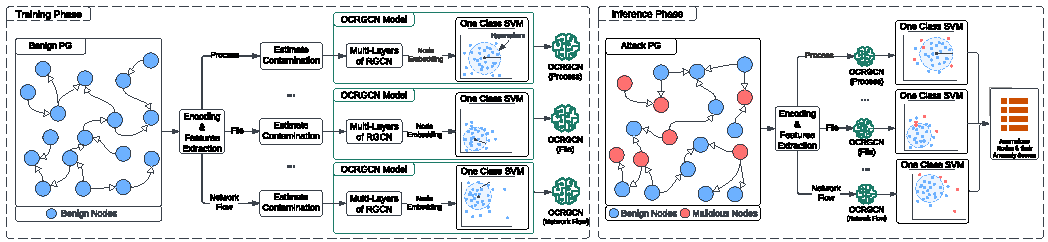
\includegraphics[width=\textwidth]{images/paper-fig2-ocrgcn.pdf}
\caption{\textbf{Ba mô hình, ba định nghĩa ``bình thường''.} \emph{Bên trái (huấn luyện):} đồ thị lành tính được mã hoá và trích đặc trưng, rồi tách theo loại nút (Process, File, Network Flow). Mỗi loại có một OCRGCN riêng: ước lượng hệ số nhiễm bẩn, qua nhiều lớp RGCN để ra embedding, rồi học một siêu cầu (khối \emph{One Class SVM}, giống Hình~\ref{fig:hypersphere}). \emph{Bên phải (suy luận):} đồ thị cần kiểm tra đi qua đúng các bước đó; mỗi nút được chấm bởi mô hình của loại mình, kết quả là danh sách nút bất thường kèm điểm. Nguồn: Hình~2 của \cite{aly2025ocrapt}.}
\figlegend{\textbf{Chú giải:} chấm xanh dương = nút lành tính; chấm đỏ = nút độc hại (chỉ có ở đồ thị kiểm tra); khung xanh lá = một mô hình OCRGCN; hình tròn trong khung \emph{One Class SVM} = siêu cầu của loại nút đó; \emph{Estimate Contamination} = ước lượng $\gamma$ (Mục~\ref{sec:theory-oneclass}); \emph{Multi-Layers of RGCN} = bộ mã hoá ở Mục~\ref{sec:theory-rgcn}.}
\label{fig:tsmod}
\end{figure}

% -----------------------------------------------------
\subsection{Xây dựng đồ thị con bất thường và lọc theo điểm (SG-Det)}
\label{sec:theory-alg1}

Nút bất thường riêng lẻ khó điều tra và có thể là dương tính giả. Thuật toán~\ref{alg:alg1} nối chúng thành các đồ thị con có quan hệ nhân quả, rồi chỉ giữ các đồ thị con đủ bất thường \tagpaper~(§5.2). Hình~\ref{fig:alg1-stages} cho thấy ý tưởng trước, thuật toán đầy đủ ở ngay sau.

\begin{figure}[H]
\centering
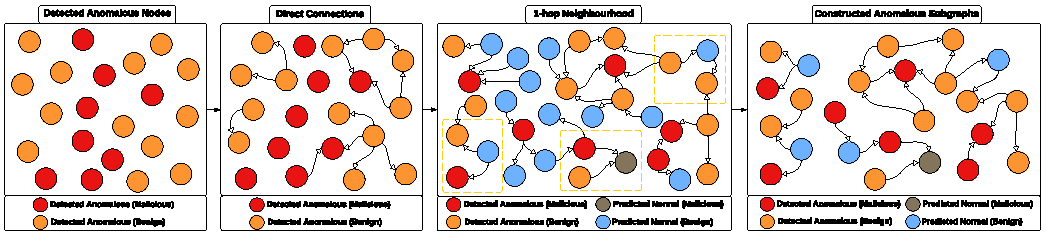
\includegraphics[width=\textwidth]{images/paper-fig3-subgraphs.pdf}
\caption{\textbf{Từ các nút rời rạc thành vài ``câu chuyện'' liên thông.} Đọc từ trái sang phải, mỗi khung là một bước của Thuật toán~\ref{alg:alg1}: (1) \emph{Detected Anomalous Nodes}: các nút bị mô hình gắn cờ, chưa nối với nhau; (2) \emph{Direct Connections}: nối các nút bất thường có cạnh trực tiếp (dòng 3); (3) \emph{1-hop Neighbourhood}: mở rộng 1 bước để thấy nút bình thường đóng vai cầu nối (dòng 4, 9); (4) \emph{Constructed Anomalous Subgraphs}: chỉ giữ đường dẫn tới nút bất thường khác, bỏ phần thừa (dòng 10--11). Nguồn: Hình~3 của \cite{aly2025ocrapt}.}
\figlegend{\textbf{Chú giải (dịch từ hình gốc):}
  \tikz[baseline=-0.6ex]\node[circle, fill=red!80!black, inner sep=2pt]{};~bị gắn cờ, thật sự độc hại\quad
  \tikz[baseline=-0.6ex]\node[circle, fill=orange!90, inner sep=2pt]{};~bị gắn cờ nhưng lành tính (dương tính giả)\quad
  \tikz[baseline=-0.6ex]\node[circle, fill=blue!45, inner sep=2pt]{};~dự đoán bình thường, đúng là lành tính\quad
  \tikz[baseline=-0.6ex]\node[circle, fill=brown!70!black, inner sep=2pt]{};~dự đoán bình thường nhưng độc hại (bỏ sót)\quad
  khung vàng nét đứt = vùng lân cận 1 bước. Ở bước cuối, nút bỏ sót (nâu) được kéo vào đồ thị con nhờ nằm giữa các nút bất thường.}
\label{fig:alg1-stages}
\end{figure}

\begin{algorithm}[H]
\caption{Xây dựng đồ thị con bất thường (theo Thuật toán 1 của \cite{aly2025ocrapt})}
\label{alg:alg1}
\begin{algorithmic}[1]
\Require Graph DB $DB_{PG}$, tập nút bất thường $A_{Nodes}$, $n_{seed}$, $max_e$
\Ensure Tập đồ thị con bất thường $A_{SGs}$
\State Truy vấn các cạnh nối trực tiếp giữa các nút trong $A_{Nodes}$ và láng giềng 1 bước của chúng; dựng $init_{SG}$
\State Sắp $A_{Nodes}$ theo điểm bất thường; $Seeds \gets$ top $n_{seed}$ nút mỗi loại
\For{mỗi $seed \in Seeds$}
  \State Duyệt $init_{SG}$ 1 bước xuôi và ngược; chỉ giữ đường dẫn tới nút bất thường chưa thăm
  \State Tạo đồ thị con $sg$
  \If{$|sg_{edges}| \le max_e$} \State thêm $sg$ vào $A_{SGs}$
  \Else \State chia $sg$ bằng Louvain thành các phần $\le max_e$ cạnh, thêm vào $A_{SGs}$
  \EndIf
\EndFor
\State Loại các đồ thị con trùng nhau
\For{mỗi $sg \in A_{SGs}$}
  \State $score(sg) \gets$ tổng điểm của các nút bất thường trong $sg$; xác định mức $sg_{ab}$
\EndFor
\State Loại các đồ thị con có mức thấp (\emph{minor})
\end{algorithmic}
\end{algorithm}

Tham số của bài báo: $n_{seed} = 15$, $max_e = 5\,000$ \tagpaper~(§7.2.1). Thuật toán Louvain \cite{blondel2008louvain} tìm cộng đồng trong đồ thị để chia đồ thị con quá lớn. Các mức bất thường theo thang logarit:

\begin{table}[H]
\centering
\begin{tabular}{l l l}
\toprule
\textbf{Điểm đồ thị con} & \textbf{Mức} & \textbf{Cảnh báo?} \\
\midrule
$< 10$ & Minor & Không \\
$10$ -- $100$ & Moderate & Có \\
$100$ -- $1\,000$ & Significant & Có \\
$> 1\,000$ & Critical & Có \\
\bottomrule
\end{tabular}
\caption{Các mức bất thường của đồ thị con trong bài báo \tagpaper~(§7.2.1). Đồ án dùng một thang khác ở mức Moderate (Mục~\ref{sec:dev-live}).}
\label{tab:levels}
\end{table}

\begin{itemize}
    \item \emph{Ví dụ 1:} một đồ thị con có 4 nút bất thường với điểm $2.5$ mỗi nút: tổng $10$, ở ranh giới Minor/Moderate. Mã nguồn gốc dùng điều kiện $> 10$ cho Moderate \tagrepo, nên đồ thị con này vẫn là Minor và bị loại.
    \item \emph{Ví dụ 2:} 30 nút với điểm $5$: tổng $150$, mức Significant, giữ lại và gửi cho bộ điều tra.
\end{itemize}
Bài báo cho thấy bỏ bước lọc này (biến thể \emph{Without SG-Det}) giữ nguyên recall nhưng làm giảm precision trên cả ba host NODLINK \tagpaper~(Bảng~4): SG-Det chủ yếu cắt dương tính giả.

% -----------------------------------------------------
\subsection{Điều tra tấn công bằng LLM}
\label{sec:theory-llm}

Bài báo nhận thấy một prompt duy nhất ``viết báo cáo từ đồ thị con'' gây ảo giác và bỏ sót giai đoạn tấn công, nên tách việc điều tra thành nhiều bước nhỏ, mỗi bước dùng prompt Chain-of-Thought \cite{wei2022cot} và được kiểm tra tự động \tagpaper~(§6, Thuật toán~2):
\begin{enumerate}
    \item \textbf{Tuần tự hoá:} mỗi đồ thị con thành một ``tài liệu log'' gồm các câu theo thời gian (\emph{chủ thể -- hành động -- đối tượng}), gộp hành động lặp lại trong cùng một giây (``read X times''); tài liệu được cắt đoạn và đánh chỉ mục trong vector store (RAG).
    \item \textbf{Trích IOC:} $\{IOC_i\} = f(ASG_{doc}, p_{ioc})$, với $f$ là lời gọi LLM và $p_{ioc}$ là prompt tương ứng.
    \item \textbf{Lọc ảo giác:} loại mọi IOC không xuất hiện trong tài liệu gốc.
    \item \textbf{Báo cáo từng đồ thị con:} $R_{atk} = f(ASG_{doc}, \{IOC_i\}', p_{sum})$; xoá bộ nhớ hội thoại sau mỗi đồ thị con.
    \item \textbf{Báo cáo tổng hợp:} trích IOC theo từng giai đoạn tấn công từ các $R_{atk}$, lọc ảo giác lần nữa, rồi tổng hợp thành $R_{comp}$.
    \item \textbf{Làm giàu:} một LLM ``giám khảo'' chọn IOC quan trọng nhất cho mỗi loại nút; truy vấn graph DB lấy ngữ cảnh 1 bước quanh IOC đó và bổ sung vào $R_{comp}$.
\end{enumerate}

\begin{figure}[H]
\centering
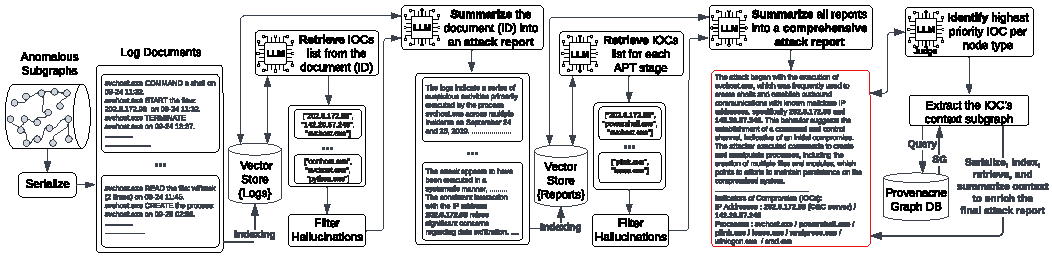
\includegraphics[width=\textwidth]{images/paper-fig4-investigator.pdf}
\caption{\textbf{Viết báo cáo theo từng bước nhỏ, mỗi bước được kiểm tra.} Đọc từ trái sang phải, khớp với 6 bước ở trên: đồ thị con được tuần tự hoá thành tài liệu log (1) và đánh chỉ mục trong vector store; LLM trích IOC (2), IOC được lọc ảo giác (3), rồi LLM tóm tắt mỗi tài liệu thành một báo cáo (4). Các báo cáo được đánh chỉ mục lần nữa, trích IOC theo giai đoạn, lọc, và gộp thành báo cáo tổng hợp (5, khung viền đỏ). Cuối cùng một LLM giám khảo chọn IOC quan trọng nhất, lấy đồ thị con ngữ cảnh từ Graph DB và bổ sung vào báo cáo (6). Đồ án dừng ở bước 5 (Mục~\ref{sec:dev-llm}). Nguồn: Hình~4 của \cite{aly2025ocrapt}.}
\figlegend{\textbf{Chú giải:} khối có biểu tượng \emph{LLM} = một lời gọi LLM với một prompt riêng; hình trụ = kho dữ liệu (vector store hoặc Graph DB); \emph{Filter Hallucinations} = bỏ IOC không có trong tài liệu gốc; \emph{Indexing} = cắt tài liệu và tính embedding để truy hồi (RAG).}
\label{fig:llm-investigator}
\end{figure}

LLM chính trong bài báo là GPT-4o-mini với temperature 0; LLaMA3-8B chạy cục bộ cho kết quả gần tương đương \tagpaper~(§7.2.2, Bảng~5). Lưu ý: bộ điều tra luôn giả định đồ thị con là một phần của tấn công; nó \emph{không} phân loại tấn công hay lành tính. Các prompt cũng đặt LLM vào vai ``người điều tra tấn công APT'' và yêu cầu báo cáo theo giai đoạn kill chain của APT \tagrepo. Mục~\ref{sec:dev-llm} mô tả cách đồ án dùng chúng cho một tấn công không phải APT.

% -----------------------------------------------------
\subsection{Cách bài báo đánh giá và các lưu ý}
\label{sec:theory-eval}

Bài báo dùng F1 làm chỉ số chính do dữ liệu mất cân bằng nặng, và tính dương tính đúng theo quy ước \emph{2 bước}: một nút độc hại được tính là phát hiện đúng nếu chính nó hoặc một láng giềng trong 2 bước bị gắn cờ \tagpaper~(§7.2). Với quy ước chặt hơn (chỉ tính nút bị gắn cờ trực tiếp), precision của OCR-APT trên TRACE giảm từ 1.00 xuống 0.87 (Bảng~6). Các lưu ý quan trọng khi đọc số liệu của bài báo:
\begin{itemize}
    \item Nhãn của DARPA TC3/OpTC được suy ra từ báo cáo ground truth dạng văn bản, không chỉ định chính xác thực thể độc hại (§7.1).
    \item Một số baseline không ổn định (ThreaTrace: F1 $0.595 \pm 0.434$ trên TC3) và kết quả của một số hệ thống lấy từ bài báo gốc của họ (§7.2).
    \item Giai đoạn tấn công bị bỏ sót trên TC3 một phần do lỗi phân tích log của hệ điều hành (§7.5).
\end{itemize}
Các số liệu này chỉ dùng để hiểu vai trò của từng thành phần; đồ án không so sánh số liệu của mình với chúng.

% =====================================================
% PHƯƠNG PHÁP TRIỂN KHAI
% =====================================================

\section{Phương pháp Triển Khai}
\label{sec:method}

Mỗi mục dưới đây nêu bài báo/mã nguồn gốc làm gì, nhóm làm gì, vì sao, và điều đó giới hạn khẳng định nào. Danh sách đầy đủ được lưu trong tài liệu sai khác (\texttt{docs/DEVIATIONS.md}, mục D1--D9) của kho mã.

% -----------------------------------------------------
\subsection{Hạ tầng lab và pipeline}
\label{sec:infra}

Phòng lab gồm hai máy ảo được dựng bằng Ansible (cấu hình theo inventory, có thể chuyển lên cloud):

\begin{table}[H]
\centering
\small
\begin{tabularx}{\textwidth}{l l X}
\toprule
\textbf{Máy} & \textbf{Hệ điều hành} & \textbf{Vai trò} \\
\midrule
\texttt{ws-etw} & Windows Server 2022 & Thu thập log nhân bằng SilkETW \cite{silketw} (Kernel-Process, Kernel-File, Kernel-Network); Grafana Alloy đẩy nguyên văn từng dòng log về Loki; workload lành tính có seed; dịch vụ web chưa vá làm mục tiêu tấn công. Không huấn luyện. \\
\texttt{ubuntu-trainer} & Ubuntu 24.04 & Loki + Grafana \cite{grafana_loki}; chuyển đổi, cắt cửa sổ, trích đặc trưng, huấn luyện; máy chủ demo trực tiếp (FastAPI + giao diện web). \\
\bottomrule
\end{tabularx}
\caption{Các máy trong phòng lab. Mọi xử lý chạy trên \texttt{ubuntu-trainer} với cùng mã chuyển đổi, bộ chuẩn hoá và danh sách quan hệ như lúc huấn luyện.}
\label{tab:vms}
\end{table}

\begin{figure}[H]
\centering
\begin{tikzpicture}[node distance=0.8cm and 0.9cm]
  % máy Windows: thu thập
  \node[prep] (etw)   at (0,0)    {SilkETW\\ \scriptsize log nhân (tiến trình, tệp, mạng)};
  \node[prep] (alloy) at (0,-1.8) {Grafana Alloy\\ \scriptsize gửi nguyên văn từng dòng};
  % máy Ubuntu: xử lý, phát hiện, hiển thị
  \node[prep] (loki) at (3.6,0)    {Loki\\ \scriptsize kho log};
  \node[prep] (s1)   at (7.0,0)    {Chuyển sang đồ thị + cắt cửa sổ 5 phút};
  \node[prep] (s2)   at (10.4,0)   {15 đặc trưng hành vi\\ \scriptsize (thang đo của tập train)};
  \node[det]  (s3)   at (10.4,-1.8) {OCRGCN theo loại nút\\ \scriptsize chấm điểm từng nút};
  \node[det]  (s4)   at (7.0,-1.8)  {Alg.~1 + lọc điểm\\ \scriptsize đồ thị con $\ge 30$?};
  \node[inv]  (s5)   at (3.6,-1.8)  {LLM: phân loại + báo cáo\\ \scriptsize (tuỳ chọn)};
  \node[outp] (ui)   at (7.0,-3.6)  {Giao diện web\\ \scriptsize cửa sổ xanh / đỏ};
  \foreach \n/\k in {s1/1, s2/2, s3/3, s4/4, s5/5} \node[num] at (\n.north west) {\k};
  % luồng dữ liệu
  \draw[arr] (etw) -- (alloy);
  \draw[arr] (alloy.east) -- node[sloped, above, font=\scriptsize]{HTTP} (loki.west);
  \draw[arr] (loki) -- (s1);
  \draw[arr] (s1) -- (s2);
  \draw[arr] (s2) -- (s3);
  \draw[arr] (s3) -- (s4);
  \draw[opt] (s4) -- (s5);
  \draw[arr] (s4) -- (ui);
  \draw[opt] (s5) |- (ui);
  % khung máy
  \begin{scope}[on background layer]
    \node[frame, fit=(etw)(alloy), label={[font=\scriptsize\ttfamily]above:ws-etw (Windows)}] {};
    \node[frame, fit=(loki)(s2)(ui)(s5), label={[font=\scriptsize\ttfamily]above:ubuntu-trainer}] {};
  \end{scope}
\end{tikzpicture}
\caption{\textbf{Cùng 5 bước như Hình~\ref{fig:ocrapt-arch}, nhưng chạy liên tục trên từng cửa sổ 5 phút.} Máy Windows chỉ thu thập và gửi log; mọi xử lý chạy trên máy Ubuntu. Đọc theo số \stepnum{1}$\to$\stepnum{5}: các số trùng với bước tương ứng của bài báo, nên có thể so từng khối. Một cửa sổ chuyển đỏ khi bước \stepnum{4} tìm được ít nhất một đồ thị con đạt mức Moderate. Luồng này dùng cho cả huấn luyện (kéo log lành tính từ Loki) và demo trực tiếp. Các điểm khác bài báo được tổng hợp ở Bảng~\ref{tab:deviations}.}
\figlegend{\textbf{Chú giải:} \swatch{cprep}{chuẩn bị dữ liệu}\quad \swatch{cdet}{phát hiện}\quad \swatch{cinv}{điều tra bằng LLM}\quad \swatch{cout}{kết quả cho người xem}\quad
  \arrowkey{arr}{luồng dữ liệu}\quad \arrowkey{opt}{tuỳ chọn}\quad
  \tikz[baseline=-0.6ex]\draw[dashed, gray, rounded corners=1pt] (0,-0.15) rectangle (0.6,0.15);~một máy ảo.}
\label{fig:our-pipeline}
\end{figure}

% -----------------------------------------------------
\subsection{Bảng tổng hợp sai khác so với bài báo}
\label{sec:dev-table}

\begin{table}[H]
\centering
\scriptsize
\renewcommand{\arraystretch}{1.25}
\begin{tabularx}{\textwidth}{>{\raggedright\arraybackslash}p{2.1cm} >{\raggedright\arraybackslash}X >{\raggedright\arraybackslash}X >{\raggedright\arraybackslash}X}
\toprule
\textbf{Thành phần} & \textbf{Bài báo / mã gốc} & \textbf{Đồ án} & \textbf{Lý do} \\
\midrule
Loại tấn công mục tiêu & APT nhiều giai đoạn (red team của DARPA, APT mô phỏng của NODLINK) & Một tấn công phổ biến: khai thác CVE của ứng dụng web trong lab $\rightarrow$ RCE $\rightarrow$ các kỹ thuật ATT\&CK & Demo trực tiếp thực tế, chạy lại được \\
Dữ liệu & DARPA TC3, OpTC, NODLINK mô phỏng & ETW tự thu thập trên Windows lab, đưa về lược đồ NODLINK W10; workload lành tính dạng script có seed & Tự làm chủ pipeline đầu--cuối cho demo; dữ liệu đủ nhỏ để kiểm tra bằng tay \\
Chế độ phát hiện & Ngoại tuyến trên toàn bộ log kiểm thử & Gần thời gian thực, cửa sổ 5 phút; mỗi nút được sao theo từng cửa sổ & Demo cần chấm điểm có giới hạn và tăng dần \\
Lưu trữ đồ thị & RDF trong GraphDB, truy vấn SPARQL & Bảng cạnh CSV, Alg.~1 chạy trong bộ nhớ cho từng cửa sổ & Một cửa sổ đủ nhỏ để nằm trong RAM \\
Đặc trưng & Bỏ cột toàn 0; chuẩn hoá idle fit trên train+test & Giữ đủ 15 cột; bộ chuẩn hoá fit trên train và dùng lại & Kích thước đặc trưng cố định; không rò rỉ dữ liệu test \\
Mô hình & OCRGCN trong bản fork PyGOD của tác giả & OCRGCN tự viết bằng \texttt{RGCNConv} của PyG, cùng siêu tham số & Hiểu và giải thích được từng dòng mã \\
Validation & 15\% ngẫu nhiên, dừng khi TNR giảm lần đầu & Giữ lại nguyên cửa sổ cuối, loại các cửa sổ chồng lấn; patience 5; seed cố định & Tránh rò rỉ giữa các cửa sổ trượt chồng nhau \\
Nhãn & Ground truth DARPA / NODLINK & Tấn công được tiêm vào và tự ghi nhãn; khớp theo chỉ dấu + thời gian & Biết chính xác cái gì đã chạy \\
Điểm đồ thị con & Tổng điểm nút (văn bản); mã gốc: tổng xác suất min-max & Tổng xác suất min-max bị kẹp $[0,1]$ theo khoảng điểm huấn luyện & Điểm thô khác thang đo giữa các loại nút \\
Mức cảnh báo & Moderate từ $>10$; lấy top-$k$ khi không có gì đạt & Moderate từ 30; không lấy top-$k$ & Cửa sổ 5 phút nhỏ hơn rất nhiều đồ thị của bài báo; top-$k$ làm mọi cửa sổ đỏ \\
LLM & Alg.~2 đầy đủ, RAG, GPT-4o-mini & Thêm bước phân loại (tấn công / lành tính / chưa rõ) trước Alg.~2 dòng 3--15; không RAG; bỏ dòng 16--25 & GNN không phân biệt được ``chưa từng thấy'' với ``độc hại''; tài liệu một cửa sổ vừa trong prompt \\
\bottomrule
\end{tabularx}
\caption{Tổng hợp các điểm đồ án làm khác bài báo. Chi tiết và tác động ở Mục~\ref{sec:dev-attack}--\ref{sec:dev-labels}.}
\label{tab:deviations}
\end{table}

% -----------------------------------------------------
\subsection{Kịch bản tấn công mục tiêu}
\label{sec:dev-attack}

\tagpaper{} OCR-APT được đánh giá trên các cuộc tấn công APT nhiều giai đoạn: tấn công của đội red team trong DARPA TC3/OpTC (kéo dài nhiều ngày) và các APT mô phỏng của NODLINK. \tagours{} Đồ án nhắm tới một tấn công phổ biến trên một máy Windows, chạy trọn trong buổi demo:
\begin{itemize}
    \item \textbf{Mục tiêu:} một ứng dụng web Next.js cố ý để chưa vá (\texttt{react2shell}), chạy trên \texttt{ws-etw}, chỉ truy cập được trong mạng lab. Lỗ hổng: \todoval[mã CVE].
    \item \textbf{Chuỗi tấn công:} khai thác ứng dụng hướng ra mạng (T1190) $\rightarrow$ thực thi lệnh qua shell (T1059) $\rightarrow$ các kỹ thuật tiếp theo: khám phá hệ thống, duy trì truy cập, đánh cắp thông tin xác thực, kênh C2, rút dữ liệu. \todoval[Mã kỹ thuật ATT\&CK cụ thể của kịch bản cuối cùng.]
    \item \textbf{Hiện trạng:} hiện mới có các kịch bản Atomic Red Team \cite{atomic_red_team} và script ATT\&CK tự viết; kịch bản CVE $\rightarrow$ RCE đang được lên kế hoạch.
\end{itemize}
\textbf{Giới hạn:} chỉ một loại tấn công trên một host, nên đồ án không khẳng định gì về khả năng phát hiện APT, tấn công nhiều host, hay tấn công trải dài nhiều ngày.

% -----------------------------------------------------
\subsection{Dữ liệu và workload lành tính}
\label{sec:dev-data}

\tagpaper{} OCR-APT được đánh giá trên các bộ dữ liệu công bố. \tagours{} Đồ án dùng dữ liệu tự thu thập vì mục tiêu là demo trực tiếp trên một máy thật:
\begin{itemize}
    \item \textbf{Thu thập:} SilkETW ghi ba provider nhân (tiến trình, tệp, mạng) dưới dạng JSON. Alloy đẩy nguyên văn từng dòng về Loki, gắn nhãn theo lần chạy và provider, nên dữ liệu huấn luyện có thể kéo lại theo lần chạy hoặc khoảng thời gian.
    \item \textbf{Chuyển đổi:} một bộ chuyển đổi đưa sự kiện ETW về đúng lược đồ NODLINK Windows 10 mà mã gốc yêu cầu (3 loại nút, 6 loại cạnh, mốc thời gian epoch mili-giây). Đồ thị được đặt tên \texttt{SimulatedW10} vì mã gốc kiểm tra tên host.
    \item \textbf{Định danh nút:} tiến trình được khoá bằng PID + thời điểm khởi động, vì Windows tái sử dụng PID và nếu chỉ dùng PID thì hai tiến trình khác nhau sẽ bị gộp, làm sai thống kê thời gian nghỉ. Tệp và luồng mạng được khoá bằng băm của đường dẫn / IP:cổng, nên định danh ổn định giữa huấn luyện và kiểm thử.
    \item \textbf{Workload lành tính:} một bộ sinh hoạt động có seed (mở trình duyệt, soạn thảo, truy cập mạng, \ldots). Ứng dụng được khởi chạy qua \texttt{explorer} (Shell COM) thay vì PowerShell, để mô hình không học ``PowerShell là cha bình thường của mọi thứ'', vì công cụ tấn công thường đi qua PowerShell.
\end{itemize}
\textbf{Tác động:} hành vi lành tính hẹp hơn người dùng thật, nên tỉ lệ dương tính giả trong lab có thể lạc quan hơn thực tế, và hoạt động nền chưa thấy lúc huấn luyện (ví dụ một tiến trình cập nhật chạy định kỳ) sẽ bị gắn cờ. \textbf{Giới hạn:} số liệu của đồ án không so sánh được với các bảng của bài báo.

% -----------------------------------------------------
\subsection{Cắt cửa sổ thời gian}
\label{sec:dev-window}

\tagpaper{} Dự đoán một lần trên toàn bộ đồ thị kiểm thử. \tagours{} Log được cắt thành các cửa sổ dài 5 phút, ký hiệu $[t, t + 5\text{ phút})$: gồm mọi sự kiện có thời điểm $\ge t$ và $< t + 5$ phút.
\begin{itemize}
    \item \emph{Huấn luyện (cửa sổ trượt, bước 2 phút):} bản ghi 20 phút bắt đầu 14:56:00 cho các cửa sổ $[14{:}56, 15{:}01)$, $[14{:}58, 15{:}03)$, $[15{:}00, 15{:}05)$, \ldots{} Một sự kiện lúc 14:59:30 thuộc cả hai cửa sổ đầu, nên các cửa sổ chồng lấn có các hàng đặc trưng tương quan.
    \item \emph{Demo (cửa sổ lật, thẳng hàng đồng hồ):} $[11{:}25, 11{:}30)$, $[11{:}30, 11{:}35)$, \ldots{} Sự kiện lúc 11:29:59.9 thuộc cửa sổ đầu; sự kiện lúc 11:30:00.0 thuộc cửa sổ sau.
\end{itemize}
\begin{figure}[H]
\centering
\begin{tikzpicture}[x=1.2cm, y=0.5cm,
  win/.style={draw, fill=cprep, rounded corners=1pt, minimum height=0.35cm},
  hit/.style={draw, fill=cdet, rounded corners=1pt, minimum height=0.35cm},
  ev/.style={circle, fill=catk, inner sep=1.5pt}]
  % (a) huấn luyện: cửa sổ trượt 5 phút, bước 2 phút; trục: phút kể từ 14:56
  \node[font=\small\bfseries, anchor=west] at (-0.2,1.6) {(a) Huấn luyện: cửa sổ trượt (dài 5 phút, bước 2 phút)};
  \draw[-{Stealth}] (0,0) -- (11.3,0);
  \foreach \m/\t in {0/14:56,2/14:58,4/15:00,6/15:02,8/15:04,10/15:06}
    {\draw (\m,0.15) -- (\m,-0.15) node[below, font=\scriptsize]{\t};}
  % đường của sự kiện vẽ trước để các thanh cửa sổ che lên; màu xanh đánh dấu cửa sổ chứa sự kiện
  \draw[catk, densely dotted, thick] (3.5,0) -- (3.5,-4.7);
  \node[hit, minimum width=6cm, anchor=west] at (0,-1.6) {\scriptsize w0000 $[14{:}56, 15{:}01)$};
  \node[hit, minimum width=6cm, anchor=west] at (2,-2.5) {\scriptsize w0001 $[14{:}58, 15{:}03)$};
  \node[win, minimum width=6cm, anchor=west] at (4,-3.4) {\scriptsize w0002 $[15{:}00, 15{:}05)$};
  \node[win, minimum width=6cm, anchor=west] at (6,-4.3) {\scriptsize w0003 $[15{:}02, 15{:}07)$};
  \node[ev, label={[font=\scriptsize, text=catk]above:14:59:30}] (e) at (3.5,0) {};
  % (b) demo: cửa sổ lật thẳng hàng đồng hồ; trục: phút kể từ 11:25
  \begin{scope}[yshift=-4.4cm]
  \node[font=\small\bfseries, anchor=west] at (-0.2,1.6) {(b) Demo trực tiếp: cửa sổ lật (dài 5 phút, nối tiếp nhau)};
  \draw[-{Stealth}] (0,0) -- (11.3,0);
  \foreach \m/\t in {0/11:25,5/11:30,10/11:35}
    {\draw (\m,0.15) -- (\m,-0.15) node[below, font=\scriptsize]{\t};}
  \node[win, minimum width=6cm, anchor=west] at (0,-1.6) {\scriptsize $[11{:}25, 11{:}30)$};
  \node[win, minimum width=6cm, anchor=west] at (5,-1.6) {\scriptsize $[11{:}30, 11{:}35)$};
  \node[ev] at (4.85,0) {}; \node[ev] at (5.15,0) {};
  \node[font=\scriptsize, text=catk, anchor=south east] at (4.85,0.15) {11:29:59.9 $\to$ cửa sổ trước};
  \node[font=\scriptsize, text=catk, anchor=south west] at (5.15,0.15) {11:30:00.0 $\to$ cửa sổ sau};
  \end{scope}
\end{tikzpicture}
\caption{\textbf{Một cửa sổ là 5 phút log được chấm điểm cùng nhau.} Ký hiệu $[t, t+5)$: gồm thời điểm $t$, không gồm $t + 5$. (a) Khi huấn luyện, các cửa sổ chồng lên nhau, nên một sự kiện (chấm đỏ lúc 14:59:30) rơi vào hai cửa sổ (tô xanh). (b) Khi demo, các cửa sổ nối tiếp không chồng lấn, nên mỗi sự kiện thuộc đúng một cửa sổ; sự kiện nằm sát ranh giới vẫn chỉ thuộc một bên.}
\figlegend{\textbf{Chú giải:} \swatch{cprep}{một cửa sổ}\quad \swatch{cdet}{cửa sổ chứa sự kiện đang xét}\quad \tikz[baseline=-0.6ex]\node[circle, fill=catk, inner sep=1.5pt]{};~một sự kiện trong log.}
\label{fig:windows}
\end{figure}

Mỗi nút được sao riêng cho từng cửa sổ (tiền tố \texttt{w0007\_}), nên thống kê thời gian nghỉ bị chặn trên bởi độ dài cửa sổ (max idle trên tập huấn luyện là 290 giây). Đồng hồ của demo là thời gian sự kiện mới nhất trừ độ trễ cho phép 20 giây (sự kiện được sắp lại theo thời gian sự kiện); khi không có log mới thì chuyển sang đồng hồ của máy chủ. Cửa sổ bắt đầu trước khi bắt đầu thu thập được đánh dấu \emph{partial} và không chấm. \textbf{Giới hạn:} không khẳng định gì về chất lượng phát hiện trên toàn bộ log; tấn công kéo dài qua ranh giới cửa sổ bị nhìn thấy từng mảnh.

% -----------------------------------------------------
\subsection{Trích đặc trưng}
\label{sec:dev-features}

\tagrepo{} Bước trích đặc trưng của mã gốc bỏ các cột toàn 0 và fit bộ chuẩn hoá min-max cho thống kê nghỉ trên cả train lẫn test. \tagours{} Đồ án viết lại bước này độc lập (không cần RDF, GraphDB hay PyG), ghi ra CSV để phân tích; giữ đủ 15 cột; fit bộ chuẩn hoá chỉ trên dữ liệu huấn luyện và dùng lại cho test và cho từng cửa sổ trực tiếp; giữ cách làm tròn khoảng nghỉ về giây như mã gốc. \textbf{Lý do:} số chiều đặc trưng phải cố định giữa huấn luyện và demo; dữ liệu test không được rò vào bộ chuẩn hoá. \textbf{Tác động:} giá trị nghỉ ở test/demo có thể vượt $[0, 1]$ (ví dụ ở Mục~\ref{sec:theory-features}). \textbf{Giới hạn:} giá trị đặc trưng không trùng khớp từng bit với mã gốc.

% -----------------------------------------------------
\subsection{Bộ huấn luyện OCRGCN}
\label{sec:dev-trainer}

\tagours{} Một OCRGCN tự viết: 3 lớp \texttt{RGCNConv}, 32 chiều, learning rate 0.005, $\beta = 0.5$ (siêu tham số của bài báo), contamination 0.001 (tức $\mathit{Min}_{con}$, vì dữ liệu huấn luyện không có nhãn). Bộ mã hoá chạy trên toàn đồ thị (12 quan hệ gồm cả quan hệ ngược), hàm mất mát chỉ tính trên các nút huấn luyện của loại đang xét. Tâm $\mathbf{c}$ và bán kính $R$ không phải tham số học: chúng được ước lượng lại trong 2 epoch khởi động ($\mathbf{c}$ là trung bình embedding, $R$ là phân vị $1 - \beta$ của khoảng cách) rồi cố định \taginf{} (theo OCGNN của PyGOD, chưa đối chiếu với bản fork của tác giả). Ngưỡng $\theta$ là phân vị $1 - \gamma$ của điểm huấn luyện.

Validation: giữ lại nguyên cửa sổ cuối cùng và loại bỏ hai cửa sổ chồng lấn với nó, thay vì chọn ngẫu nhiên 15\% số nút như mã gốc, vì với cửa sổ trượt thì cùng một hành vi xuất hiện ở nhiều cửa sổ và chia ngẫu nhiên sẽ rò rỉ. Dừng sớm theo patience 5 epoch thay vì dừng ngay lần đầu TNR giảm; seed cố định (360 + chỉ số lần chạy). \textbf{Giới hạn:} không thể khẳng định đã tái hiện chính xác OCRGCN của tác giả.

% -----------------------------------------------------
\subsection{Đường chạy trực tiếp, Thuật toán 1 và thang mức cảnh báo}
\label{sec:dev-live}

Mỗi cửa sổ đóng lại được chấm bằng bộ chuẩn hoá, danh sách quan hệ và các mô hình đã đông cứng từ lúc huấn luyện; quan hệ chưa từng thấy lúc huấn luyện bị bỏ (có đếm). Sau đó Thuật toán~\ref{alg:alg1} chạy trong bộ nhớ, bám theo mã gốc \tagrepo: $n_{seed} = 15$, đồ thị con có ít nhất 3 nút, mỗi nút chỉ được gom một lần, Louvain khi vượt 5\,000 cạnh, loại đồ thị con trùng.

\paragraph{Điểm đồ thị con.}
\tagpaper{} Văn bản bài báo nói điểm đồ thị con là ``tổng điểm'' của các nút bất thường. Nhưng điểm thô $s_i$ có thang khác nhau giữa các loại nút (của NET có thể âm), nên cộng thẳng không có nghĩa. \tagrepo{} Mã gốc cộng \emph{xác suất} min-max của PyGOD. Đồ án làm theo mã gốc:
\[
p_i = \operatorname{clamp}\!\left(\frac{s_i - s^{train}_{\min,\tau}}{s^{train}_{\max,\tau} - s^{train}_{\min,\tau}},\ 0,\ 1\right), \qquad score(sg) = \sum_{i \in sg,\ i \text{ bất thường}} p_i ,
\]
với $s^{train}_{\min,\tau}, s^{train}_{\max,\tau}$ là điểm nhỏ nhất/lớn nhất của loại nút $\tau$ trên tập huấn luyện; $\operatorname{clamp}(x, 0, 1)$ cắt $x$ về khoảng $[0, 1]$.
\begin{itemize}
    \item \emph{Ví dụ 1:} loại FILE có điểm huấn luyện trong $[0.10, 0.23]$. Một tệp có $s = 0.32$: $(0.32 - 0.10)/(0.23 - 0.10) \approx 1.69$, kẹp về $p = 1$.
    \item \emph{Ví dụ 2:} một tệp có $s = 0.165$: $(0.165 - 0.10)/0.13 = 0.5$. Một đồ thị con gồm 18 tệp kiểu Ví dụ 1 có điểm $18$; vì $p \le 1$, điểm $\ge 30$ nghĩa là \emph{ít nhất khoảng 30 nút bất thường trong cùng một câu chuyện liên thông}.
\end{itemize}

\paragraph{Thang mức cảnh báo.}
\tagours{} Cửa sổ chỉ chuyển đỏ nếu có ít nhất một đồ thị con đạt Moderate, với Moderate bắt đầu từ 30 (mã gốc: $> 10$); các mốc khác giữ nguyên. Lý do: bài báo nói tập đồ thị con ``có thể điều chỉnh theo ngưỡng bất thường mong muốn'' (§5.2), và một cửa sổ 5 phút (khoảng 100--850 nút) nhỏ hơn rất nhiều đồ thị cỡ DARPA mà các mức được đặt ra \taginf. Mốc 30 được chọn từ \emph{một} cửa sổ lành tính duy nhất trong lần chạy thử: một tiến trình cập nhật chưa thấy lúc huấn luyện nạp 18 DLL, cho điểm 18 (vượt mốc 10 của mã gốc). Thang này \emph{che} dương tính giả đó chứ không sửa nó; cách sửa thật là mở rộng dữ liệu huấn luyện lành tính. Đồ án cũng \emph{không} dùng cơ chế lấy top-$k$ của mã gốc khi không có đồ thị con nào đạt Moderate, vì khi chạy trực tiếp điều đó làm mọi cửa sổ đều đỏ. \textbf{Giới hạn:} mốc 30 là của nhóm, đặt trên dữ liệu lành tính, chưa kiểm chứng trên tấn công; không được chỉnh lại mốc dựa trên chính cửa sổ tấn công (Mục~\ref{sec:res-attack}).

% -----------------------------------------------------
\subsection{Bước LLM: phân loại trước, báo cáo sau}
\label{sec:dev-llm}

\tagpaper{} Thuật toán 2 coi mọi đồ thị con là một phần của tấn công và không bao giờ phân loại. \tagours{} Với mỗi cửa sổ đỏ, một prompt trung lập trước hết trả về kết luận dạng JSON (\emph{attack} / \emph{benign} / \emph{uncertain}, các tactic ATT\&CK, các dòng bằng chứng). Prompt này không giả định APT và dùng tactic ATT\&CK thay cho giai đoạn kill chain của APT, phù hợp với tấn công mục tiêu (Mục~\ref{sec:dev-attack}). Dòng bằng chứng phải xuất hiện nguyên văn trong tài liệu, nếu không kết luận bị hạ thành \emph{uncertain}. Chỉ khi kết luận là \emph{attack} thì mới chạy các prompt của bài báo (sao nguyên văn từ mã gốc): trích IOC $\rightarrow$ lọc ảo giác $\rightarrow$ báo cáo từng đồ thị con $\rightarrow$ (nếu có $\ge 2$ đồ thị con tấn công) IOC theo giai đoạn $\rightarrow$ báo cáo tổng hợp, tức Thuật toán~2 dòng 3--15. Các prompt này vẫn giữ nguyên cách gọi ``APT'' của bài báo; báo cáo vì thế có thể dùng từ ngữ APT cho một tấn công không phải APT.
\begin{itemize}
    \item Không dùng vector store: tài liệu của một cửa sổ vừa trong prompt; tài liệu dài hơn 400 dòng bị cắt, ưu tiên các dòng chạm nút bất thường.
    \item Bỏ dòng 16--25 (LLM giám khảo chọn IOC, truy vấn graph DB, làm giàu báo cáo).
    \item Tuần tự hoá theo mã gốc, nhưng dùng thời gian UTC thật, đường dẫn đầy đủ, và giải mã địa chỉ mạng của SilkETW (lưu dưới dạng số nguyên có dấu) chỉ để hiển thị.
    \item Nhà cung cấp LLM thay được (Anthropic, OpenAI, Ollama, hoặc một bộ giả lập theo từ khoá chỉ dùng để kiểm thử giao diện).
\end{itemize}
Kết luận của LLM là một lớp phủ: không bao giờ xoá cảnh báo của GNN (cửa sổ vẫn đỏ, nhãn \emph{false positive} hiển thị gạch ngang), và không bao giờ được đưa ngược vào huấn luyện, vì nội dung log (đường dẫn, tên tiến trình) do kẻ tấn công kiểm soát được nên có thể bị prompt injection, và mô hình mối đe doạ giả định log huấn luyện sạch. \textbf{Giới hạn:} chưa khẳng định LLM phân biệt được tấn công với dương tính giả cho tới khi chạy trên cửa sổ có nhãn; không so sánh chất lượng báo cáo với Bảng~5 của bài báo.

% -----------------------------------------------------
\subsection{Nhãn từ tấn công được tiêm vào}
\label{sec:dev-labels}

\tagpaper{} Ground truth từ DARPA/NODLINK (với các lưu ý ở Mục~\ref{sec:theory-eval}). \tagours{} Các kịch bản tấn công (Atomic Red Team \cite{atomic_red_team} và kịch bản tự viết, chạy song song với workload lành tính) tự ghi một tệp JSONL nhãn; một nút được coi là độc hại nếu khớp một chỉ dấu (tên tiến trình, đường dẫn, địa chỉ) \emph{và} hoạt động trong khoảng thời gian của tấn công. Đây là một ``oracle'' yếu: tiến trình lành tính trùng tên trong cùng khoảng thời gian có thể bị gán nhãn độc hại nhầm. \textbf{Giới hạn:} chỉ khẳng định được ``phát hiện các kỹ thuật ATT\&CK được tiêm vào trên dữ liệu của nhóm''.

% -----------------------------------------------------
\subsection{Những khẳng định đồ án không đưa ra}
\label{sec:claims}
\begin{itemize}
    \item Không so sánh precision/recall/F1 của nhóm với Bảng~2--4 của bài báo: dữ liệu, nhãn, quy ước tính và chế độ phát hiện đều khác.
    \item Không khẳng định chất lượng phát hiện trước khi có cửa sổ được gán nhãn; một cửa sổ là một điểm dữ liệu, không phải một tỉ lệ.
    \item Không khẳng định tái hiện chính xác OCRGCN, Thuật toán 1 dựa trên GraphDB, hay Thuật toán 2 đầy đủ.
    \item Nếu có báo cáo số liệu: seed cố định, nhiều lần chạy, trung bình $\pm$ độ lệch chuẩn, và ghi rõ nguồn nhãn.
\end{itemize}

% =====================================================
% KẾT QUẢ
% =====================================================

\section{Kết Quả Thực Nghiệm và Đánh Giá}
\label{sec:results}

% TODO: điền sau khi có lần huấn luyện mới (dữ liệu lành tính mở rộng, kéo từ Loki) và các phiên demo.
Mô hình dùng cho các thí nghiệm: \todoval[tên run, ngày huấn luyện, số cửa sổ/cạnh/nút lành tính theo từng loại, seed]. Mọi thí nghiệm dùng cùng một mô hình, bộ chuẩn hoá và danh sách quan hệ.

% -----------------------------------------------------
\subsection{R1 -- Các cửa sổ lành tính}
\label{sec:res-benign}

\paragraph{Câu hỏi và giả thuyết.}
Trả lời RQ1. Với hoạt động lành tính (workload có seed và hoạt động nền của hệ điều hành), không đồ thị con nào đạt Moderate ($score \ge 30$), nên mọi cửa sổ giữ màu xanh.

\paragraph{Thiết lập.}
\todoval[Số phiên demo lành tính, thời điểm trong ngày, độ dài mỗi phiên, tác vụ nền được kích hoạt (ví dụ trình cập nhật, quét Defender)]. Mỗi phiên được chấm trực tiếp và chấm lại ngoại tuyến từ log đã lưu với cùng mô hình.

\begin{table}[H]
\centering
\small
\begin{tabular}{l r r r r l}
\toprule
\textbf{Phiên} & \textbf{\# cửa sổ} & \textbf{\# cửa sổ có nút $> \theta$} & \textbf{\# nút $> \theta$ (P/F/N)} & \textbf{Max $score(sg)$} & \textbf{Mức cao nhất} \\
\midrule
\todoval & \todoval & \todoval & \todoval & \todoval & \todoval \\
\todoval & \todoval & \todoval & \todoval & \todoval & \todoval \\
\todoval & \todoval & \todoval & \todoval & \todoval & \todoval \\
\midrule
\textbf{Tổng / TB $\pm$ std} & \todoval & \todoval & \todoval & \todoval & -- \\
\bottomrule
\end{tabular}
\caption{Kết quả trên các phiên lành tính. P/F/N: số nút PROCESS/FILE/NET vượt ngưỡng. Max $score(sg)$: điểm đồ thị con lớn nhất trong phiên.}
\label{tab:res-benign}
\end{table}

\begin{figure}[H]
\centering
\fbox{\parbox[c][4cm][c]{0.9\textwidth}{\centering \todoval[Ảnh chụp dòng thời gian cửa sổ trên giao diện demo (xanh/đỏ)]}}
\caption{Dòng thời gian các cửa sổ của một phiên lành tính.}
\label{fig:res-benign}
\end{figure}

\paragraph{Nhận xét.}
\todoval[Nhóm bổ sung: các nút vượt ngưỡng là gì, vì sao (hoạt động nền chưa thấy lúc huấn luyện?), khoảng cách giữa max điểm lành tính và mốc 30.]

\paragraph{Giới hạn của R1.}
\begin{itemize}
    \item Dữ liệu lành tính là workload dạng script trên một máy, hẹp hơn người dùng thật.
    \item Mốc 30 được chọn từ dữ liệu lành tính; R1 kiểm tra nó trên các phiên khác nhưng vẫn cùng một môi trường.
\end{itemize}

% -----------------------------------------------------
\subsection{R2 -- Tấn công chạy trực tiếp trong lúc demo}
\label{sec:res-attack}

\paragraph{Câu hỏi và giả thuyết.}
Trả lời RQ2. Cửa sổ chứa tấn công có ít nhất một đồ thị con đạt Moderate, và đồ thị con đó chứa các thực thể của tấn công (ví dụ dịch vụ web sinh ra shell, tệp được thả, kết nối ra ngoài).

\paragraph{Thiết lập.}
Kịch bản (Mục~\ref{sec:dev-attack}): khai thác lỗ hổng \todoval[mã CVE] trên ứng dụng web chưa vá trong lab (\texttt{react2shell}) $\rightarrow$ thực thi mã từ xa $\rightarrow$ khám phá hệ thống, duy trì truy cập, đánh cắp thông tin xác thực, kênh C2, rút dữ liệu \todoval[mã kỹ thuật ATT\&CK và thời điểm từng bước]. Tấn công chạy song song với workload lành tính và tự ghi nhãn (Mục~\ref{sec:dev-labels}). Mốc Moderate giữ nguyên 30 như đã đặt trên dữ liệu lành tính; \emph{không} chỉnh mốc theo cửa sổ tấn công, vì như vậy là khớp ngưỡng theo dữ liệu kiểm thử.

\begin{table}[H]
\centering
\small
\begin{tabularx}{\textwidth}{l r l X X}
\toprule
\textbf{Cửa sổ} & \textbf{$score(sg)$} & \textbf{Mức} & \textbf{Nút bất thường chính} & \textbf{Chỉ dấu tấn công khớp / tổng} \\
\midrule
\todoval & \todoval & \todoval & \todoval & \todoval \\
\todoval & \todoval & \todoval & \todoval & \todoval \\
\bottomrule
\end{tabularx}
\caption{Các cửa sổ trong khoảng thời gian tấn công.}
\label{tab:res-attack}
\end{table}

\begin{figure}[H]
\centering
\fbox{\parbox[c][5cm][c]{0.9\textwidth}{\centering \todoval[Ảnh đồ thị con cảnh báo trên giao diện demo]}}
\caption{Đồ thị con bất thường của cửa sổ tấn công.}
\label{fig:res-attack}
\end{figure}

\paragraph{Nhận xét.}
\todoval[Nhóm bổ sung: tấn công có làm cửa sổ chuyển đỏ không; điểm so với mốc 30; tấn công có bị cắt qua hai cửa sổ không; nút độc hại nào bị bỏ sót và vì sao.]

\paragraph{Giới hạn của R2.}
\begin{itemize}
    \item Một kịch bản, \todoval[số] lần chạy: chứng minh khái niệm, không phải tỉ lệ phát hiện.
    \item Nhãn từ oracle chỉ dấu + thời gian, không phải ground truth của chuyên gia phân tích.
\end{itemize}

% -----------------------------------------------------
\subsection{R3 -- Phân loại và báo cáo bằng LLM}
\label{sec:res-llm}

\paragraph{Câu hỏi và giả thuyết.}
Trả lời RQ3. Với cửa sổ tấn công ở R2, LLM kết luận \emph{attack} và báo cáo nêu được các IOC và giai đoạn chính; với các cửa sổ đỏ lành tính (nếu có), LLM kết luận \emph{benign} hoặc \emph{uncertain}.

\paragraph{Thiết lập.}
Nhà cung cấp và mô hình: \todoval. Số lần chạy lại mỗi cửa sổ: \todoval{} (với các mô hình không đặt được temperature thì kết quả không tất định).

\begin{table}[H]
\centering
\small
\begin{tabular}{l l l l r r}
\toprule
\textbf{Cửa sổ} & \textbf{Nhãn thật} & \textbf{Kết luận LLM} & \textbf{Tactic ATT\&CK} & \textbf{IOC đúng / IOC trích} & \textbf{\# lời gọi} \\
\midrule
\todoval & \todoval & \todoval & \todoval & \todoval & \todoval \\
\todoval & \todoval & \todoval & \todoval & \todoval & \todoval \\
\bottomrule
\end{tabular}
\caption{Kết luận của LLM trên các cửa sổ đỏ.}
\label{tab:res-llm}
\end{table}

\begin{lstlisting}[caption={Trích đoạn báo cáo tấn công do LLM sinh ra (điền sau).}, label={lst:report}]
[TODO: paste report excerpt: summary, attack stages, IOCs, timeline]
\end{lstlisting}

\paragraph{Nhận xét.}
\todoval[Nhóm bổ sung: IOC có bị ảo giác không; giai đoạn nào bị bỏ sót; LLM có đưa ra kết luận sai không.]

\paragraph{Giới hạn của R3.}
\begin{itemize}
    \item Số cửa sổ đỏ ít; kết luận của LLM không phải ground truth.
    \item Thuộc tính tiến trình chỉ có tên ảnh (không có dòng lệnh), nên LLM có ít ngữ cảnh cho nút tiến trình.
\end{itemize}

% =====================================================
% THẢO LUẬN VÀ KẾT LUẬN
% =====================================================

\section{Thảo luận, Hạn chế và Kết Luận}
\label{sec:conclusion}

\paragraph{Đóng góp của đồ án.}
\begin{itemize}
    \item Một pipeline tự xây dựng, kiểm tra được từng bước, từ log ETW của Windows tới lược đồ NODLINK, đặc trưng hành vi, OCRGCN theo loại nút, Thuật toán~1 và một phần Thuật toán~2.
    \item Chạy OCR-APT theo cửa sổ gần thời gian thực, với cùng mã cho huấn luyện và demo.
    \item Bước phân loại bằng LLM trước khi viết báo cáo, thứ mà bài báo không có.
    \item Một bản ghi trung thực các sai khác và giới hạn của từng sai khác.
\end{itemize}

\paragraph{Hạn chế đã biết.}
\begin{itemize}
    \item Dữ liệu lành tính hẹp; hoạt động nền chưa thấy lúc huấn luyện bị gắn cờ, và thang mức Moderate $\ge 30$ chỉ che dương tính giả đó.
    \item Ngưỡng nút $\theta$ nằm sát điểm huấn luyện lớn nhất (contamination 0.001), nên bất kỳ nút lành tính nào trong một ngữ cảnh mới đều dễ vượt ngưỡng.
    \item Cửa sổ 5 phút cắt rời hành vi kéo dài; một tấn công có các bước rải ra nhiều cửa sổ có thể không đạt Moderate ở cửa sổ nào.
    \item Chỉ trình diễn một loại tấn công trên một host; không khẳng định gì về APT hay tấn công nhiều host.
    \item Mốc 30 được đặt từ một cửa sổ lành tính và chưa kiểm chứng trên tấn công.
\end{itemize}

\paragraph{Kết luận.}
\todoval[Tóm tắt câu trả lời cho RQ1--RQ3 và hướng phát triển: mở rộng dữ liệu lành tính, hiệu chỉnh ngưỡng trên nhiều phiên, cửa sổ trượt cho tấn công vượt ranh giới, thêm kịch bản tấn công.]
